% !TeX root=debugging.tex

\subsection{Approaches}

\begin{frame}
    \frametitle{How to debug}
    \begin{figure}
        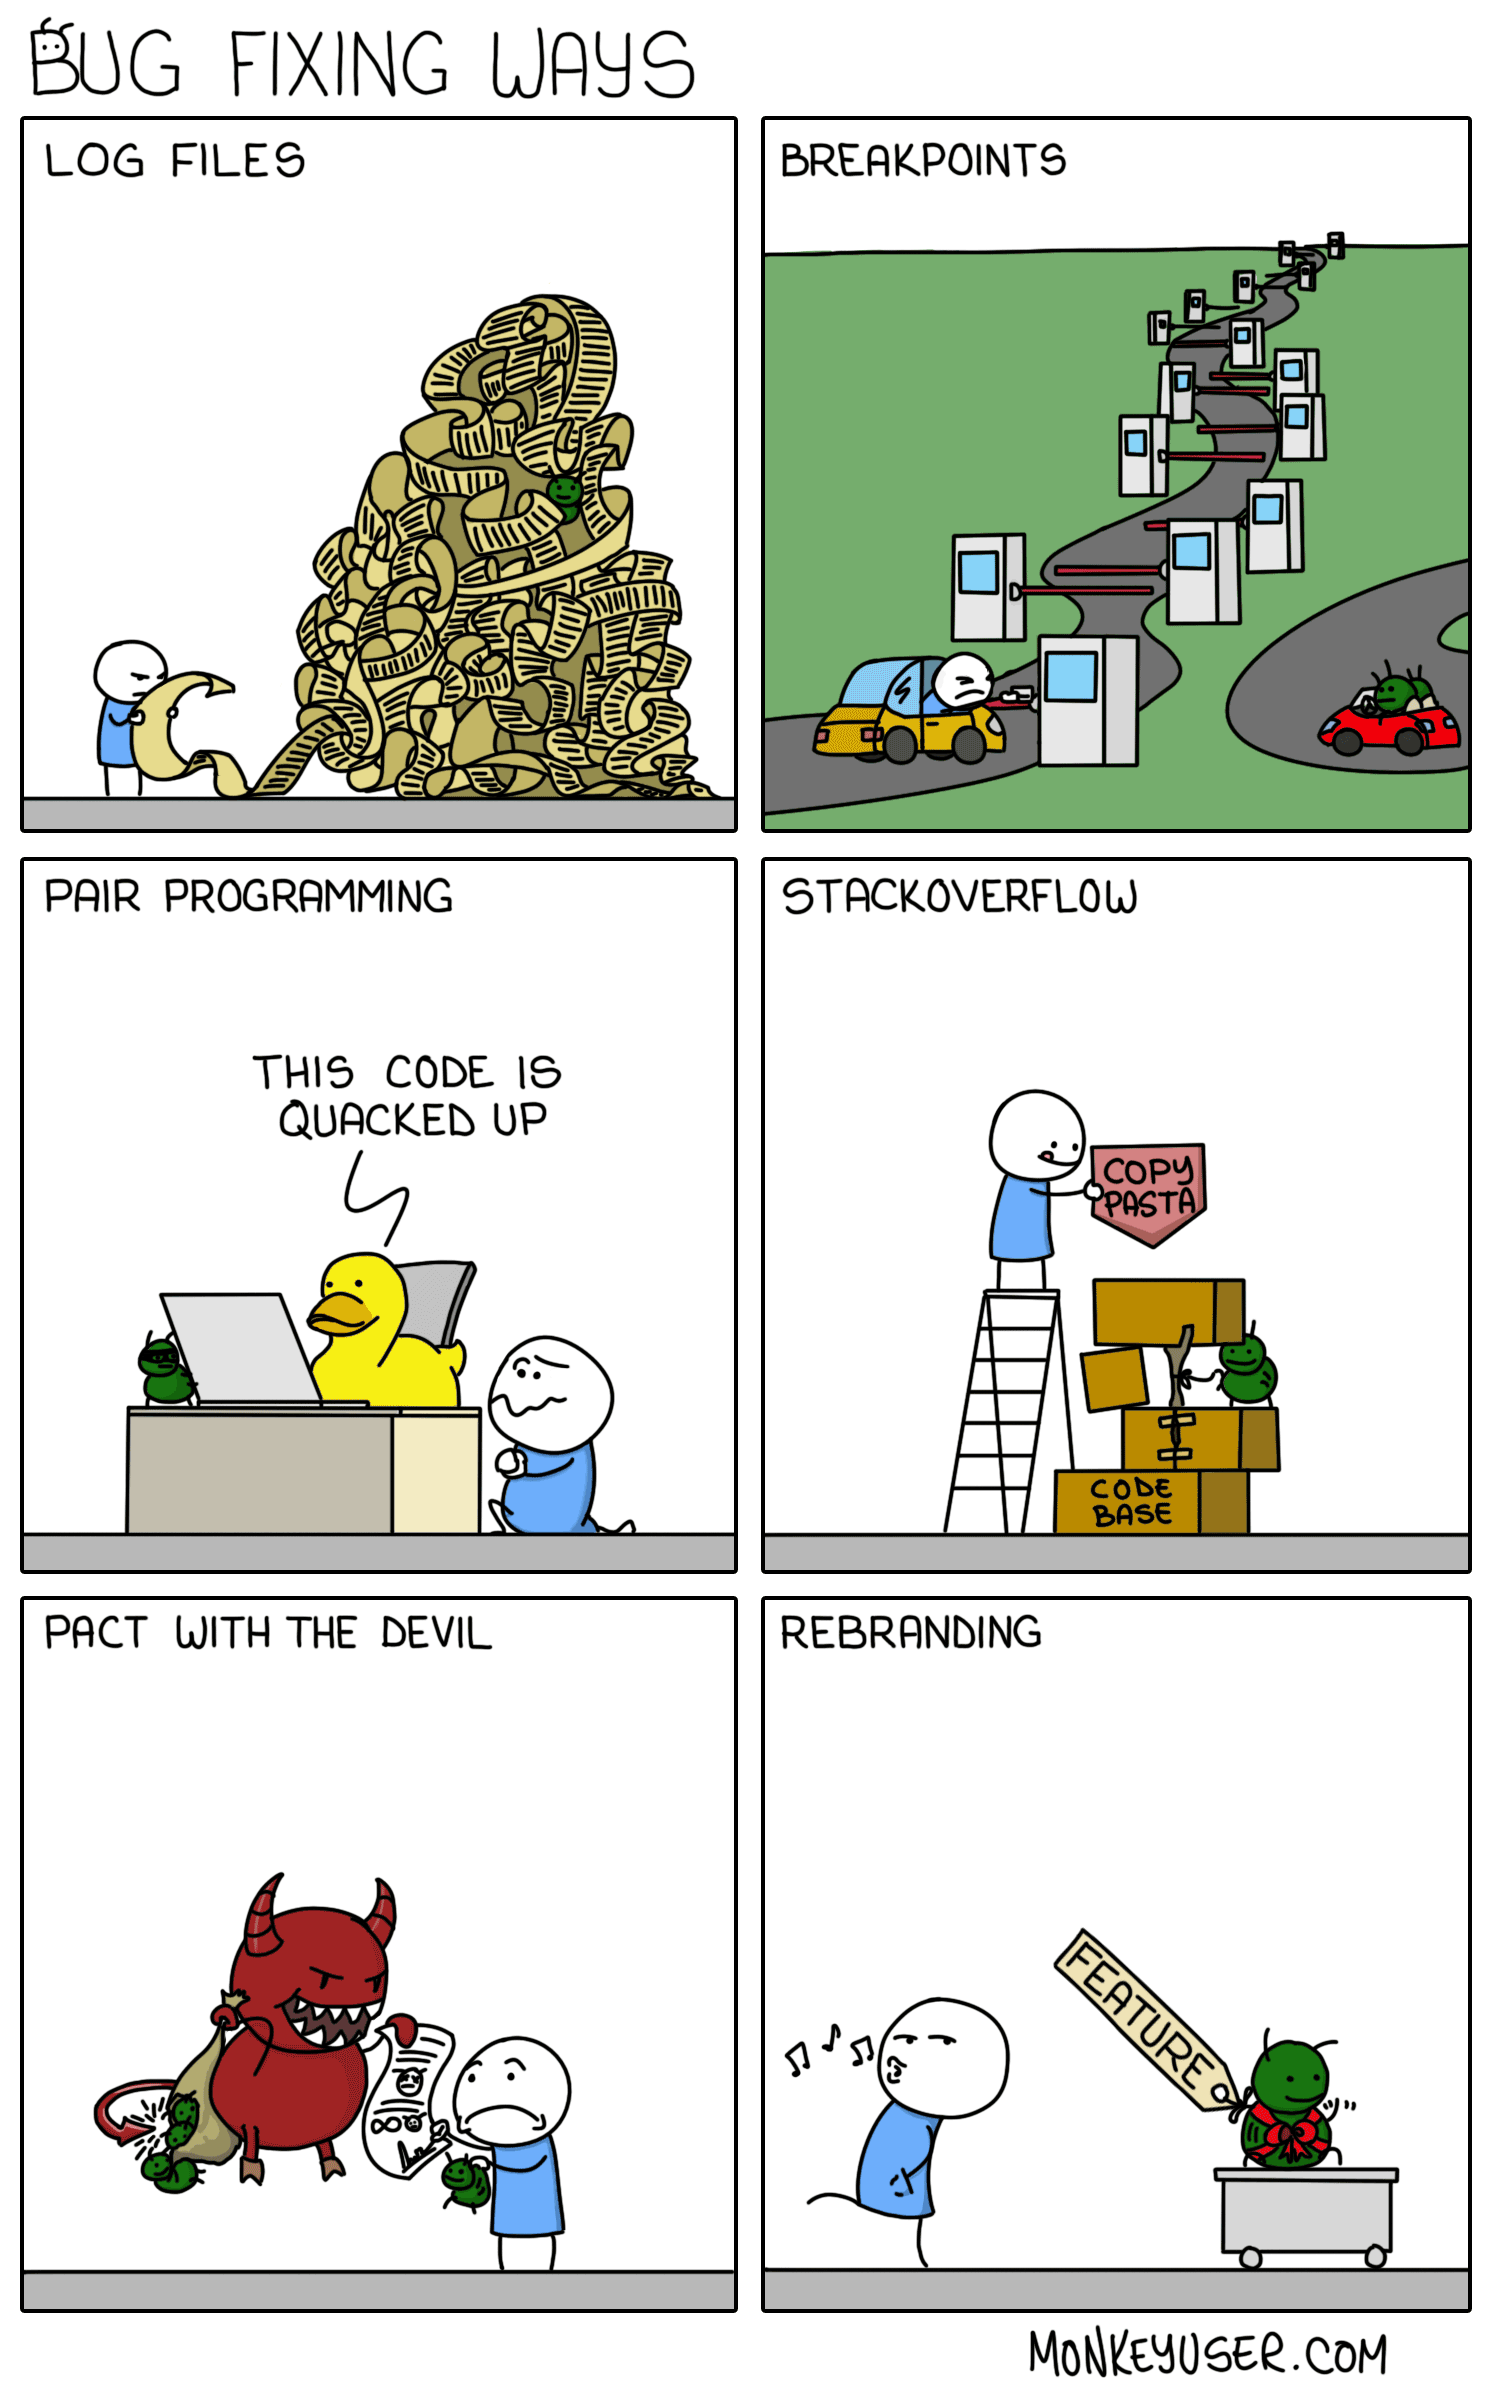
\includegraphics[height=0.8\textheight]{bug-fixing-ways.png}
    \end{figure}
\end{frame}

\begin{frame}
    \frametitle{False assumptions}
    \tikz[overlay]\node[anchor=east] at (70ex,8ex) {\tiny\href{https://sway.office.com/PavDhCql8Adms1Ap}{\textit{The Art of Debugging}}, Ehsan Hajyasini, UT AP F96};
    Finding your bug is a process of confirming the many things you believe are true, until you find one which is not true.
    \onslide<+->
    \begin{itemize}[<+->]
        \item you believe that at a certain point in your source file, a certain \textbf{variable} has a certain \textbf{value}
        \item you believe that in a given \texttt{if-then-else} statement, the \texttt{else} \textbf{branch} is the one that is \textbf{executed}
        \item you believe that when you call a certain function, the \textbf{function} \textbf{receives} its \textbf{parameters} correctly
    \end{itemize}
    \onslide<+->So\dots check the assumptions!\onslide<+-> $\longrightarrow$ binary search\onslide<+->, pre \& post conditions
\end{frame}

\begin{frame}<beamer:0>
    \frametitle{More examples of false assumptions}
    \tikz[overlay]\node[anchor=east] at (70ex,1ex) {\tiny\href{https://jvns.ca/blog/2019/06/23/a-few-debugging-resources/}{\textit{What does debugging a program look like?}}, Julia Evans};
    \begin{itemize}[<+->]
        \item this variable is set to X (``that filename is definitely right'')
        \item that variable's value can't possibly have changed between X and Y
        \item this code was doing the right thing before
        \item this function does X
        \item I'm editing the right file
        \item there can't be any typos in that line I wrote it is just 1 line of code
        \item the documentation is correct
        \item the code I'm looking at is being executed at some point
        \item these two pieces of code execute sequentially and not in parallel
        \item the code does the same thing when compiled in debug / release mode (or with \texttt{-O2} and without, or\ldots)
        \item the compiler is not buggy\onslide<+->{} (though this is last on purpose, the compiler is only very rarely to blame :) )
    \end{itemize}
\end{frame}

\begin{frame}
    \frametitle{Stabilize, isolate, minimize}
    \tikz[overlay]\node[anchor=east] at (70ex,14ex) {\tiny\href{https://sway.office.com/PavDhCql8Adms1Ap}{\textit{The Art of Debugging}}, Ehsan Hajyasini, UT AP F96};
    \begin{itemize}[<+->]
        \item make failure-inducing \textbf{input smaller} \onslide<+->$\longrightarrow$ is more relevant\onslide<+->, saves time
        \item make the program \textbf{crash faster}
        \item make the situation \textbf{deterministic} \onslide<+->$\longrightarrow$ make bugs \textbf{reproducible}
    \end{itemize}
\end{frame}

\begin{frame}
    \frametitle{Reproducing bugs}
    \begin{figure}
        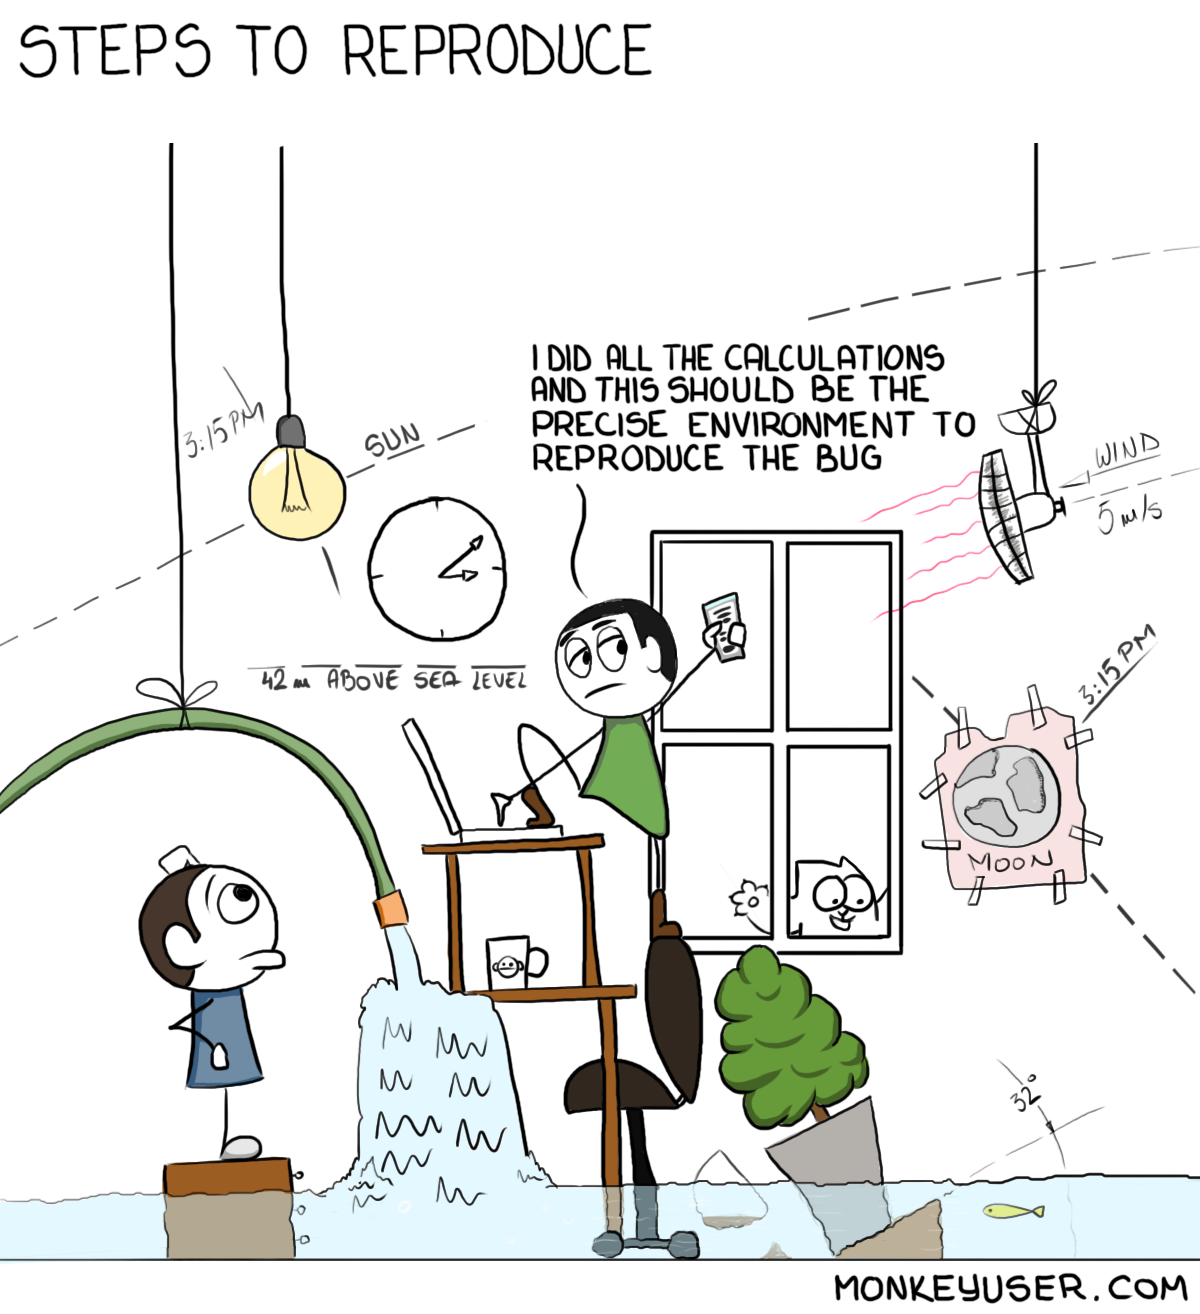
\includegraphics[height=0.8\textheight]{steps-to-reproduce.png}
    \end{figure}
\end{frame}

\begin{frame}<beamer:0>
    \frametitle{Reproducing bugs}
    \tikz[overlay]\node[anchor=east] at (70ex,10ex) {\tiny\href{https://jvns.ca/blog/2019/06/23/a-few-debugging-resources/}{\textit{What does debugging a program look like?}}, Julia Evans};
    \begin{itemize}[<+->]
        \item for something that requires clicking on a bunch of things in a browser to reproduce, recording what you clicked on with \textit{Selenium} and getting \textit{Selenium} to replay the UI interactions
        \item writing a unit test that reproduces the bug\onslide<+->\\\textbf{bonus}: you can add this to your test suite later if it makes sense
        \item writing a script or finding a command line incantation that does it
    \end{itemize}
\end{frame}

\begin{frame}<beamer:0>
    \frametitle{Scientific method of debugging}
    \tikz[overlay]\node[anchor=east] at (58ex,5ex) {\tiny\textit{Debugging}, Max Goldman and Rob Miller, \href{http://web.mit.edu/6.031/www/fa17/}{MIT Software Construction (6.031) F17}};
    \tikz[overlay]\node[rotate=-6] at (63ex,4.5ex) {
\includegraphics[width=0.13\textwidth]{whyprogramsfail.jpg}};
    \begin{enumerate}[<+->]
        \item \textbf{study the data} \onslide<+->$\longrightarrow$ incorrect results\onslide<+->, failed assertions\onslide<+->, stack traces
        \item \textbf{hypothesize} \onslide<+->$\longrightarrow$ where the bug might be\onslide<+->, or where it cannot be
            \begin{itemize}[<+->]
                \item \textbf{slicing} \onslide<+->$\longrightarrow$ When you have a failure the \textit{slice} for that value consists of the lines of the program that helped compute the bad value.
                \item \textbf{delta debugging} \onslide<+->$\longrightarrow$ difference between successful execution and failing execution\onslide<+->: test cases\onslide<+->, \href{https://martinfowler.com/bliki/DiffDebugging.html}{diff debugging} \& undoing changes 
                \item \textbf{swap components} \onslide<+->$\longrightarrow$ different implementations
            \end{itemize}
            \onslide<+->\textbf{prioritizing hypotheses} \onslide<+->$\longrightarrow$ old, well-tested code vs recently-added code\onslide<+->, library code vs your code
        \item \textbf{experiment} \onslide<+->$\longrightarrow$ devise and run an experiment 
        \item \textbf{repeat}
    \end{enumerate}
\end{frame}
